\documentclass{article}
\usepackage[utf8]{inputenc}

\title{Normalizacion}
\author{Alejandro Iabin Arteaga Hernández}
\date{Diciembre 2019}

\usepackage{natbib}
\usepackage{graphicx}

\begin{document}

\maketitle

\section{Modelo relacional sin normalizar}
\begin{figure}[h!]
\centering
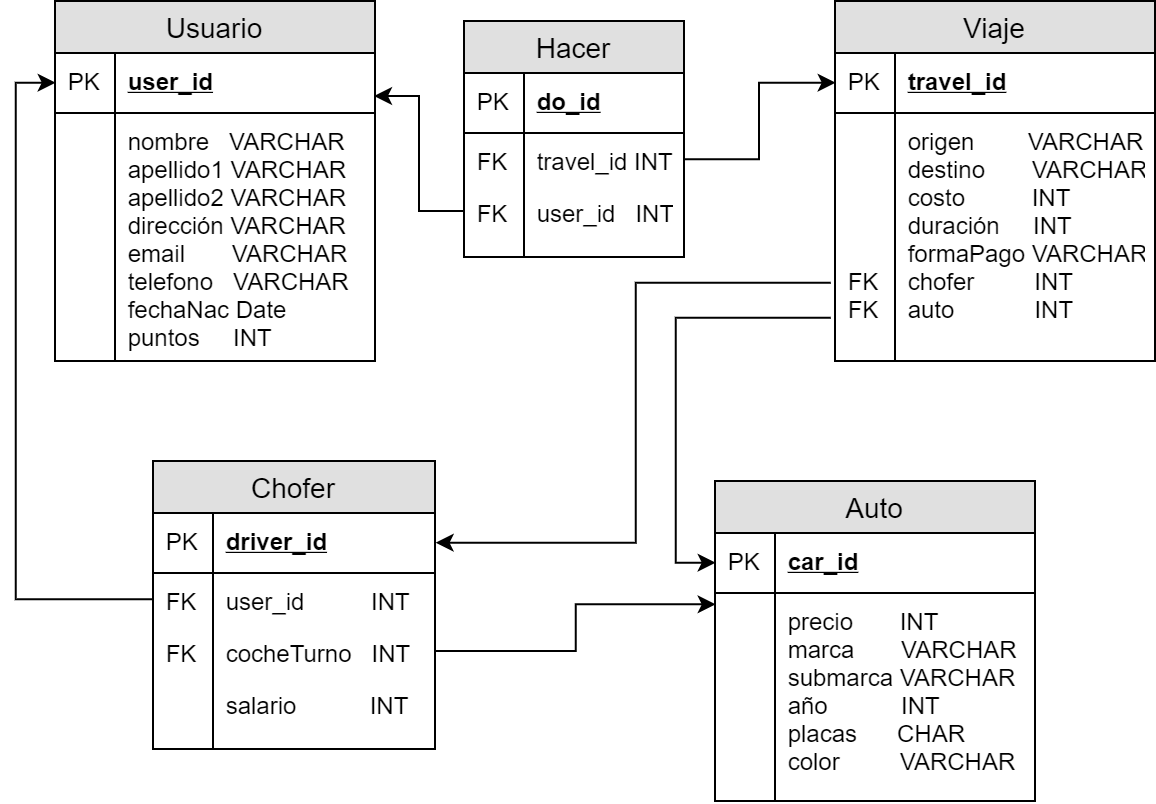
\includegraphics[scale=0.32]{sin.png}
\caption{Diagrama relacional sin normalizar}
\end{figure}
\newpage
\section{Primera forma normal}
Una relación está en forma normal si
\begin{itemize}
    \item Todos los atributos son atómicos. Un atributo es atómico si los elementos del dominio son simples e indivisibles.
    \item No debe existir variación en el número de columnas.
    \item Los campos no clave deben identificarse por la clave (dependencia funcional).
    \item Debe existir una independencia del orden tanto de las filas como de las columnas; es decir, si los datos cambian de orden no deben cambiar sus significados.
\end{itemize}
Así que debemos comenzar a analizar si nuestro modelo relacional cumple las reglas de la 1NF.\par\null\par
Todos los atributos de cada tabla son atómicos, ya que nos encargamos de expandir los atributos multivaluados cuando se hizo el diagrama relacional. \par\null\par
No existe variación en el número de columnas, ya que todos las filas deben tener los mismo datos\par\null\par
Existe una independencia del orden de las filas, este no afecta a la semántica de cada tabla, eso se cumple\par\null\par
Lo único que no se cumple es que no todos los campos son dependencia funcional de la llave primaria, por ejemplo, un usuario puede tener muchos teléfonos y muchos emails, entonces el teléfono y el email no es dependencia funcional de la llave primaria, debemos cambiar eso.\par\null\par
\begin{figure}[h!]
\centering
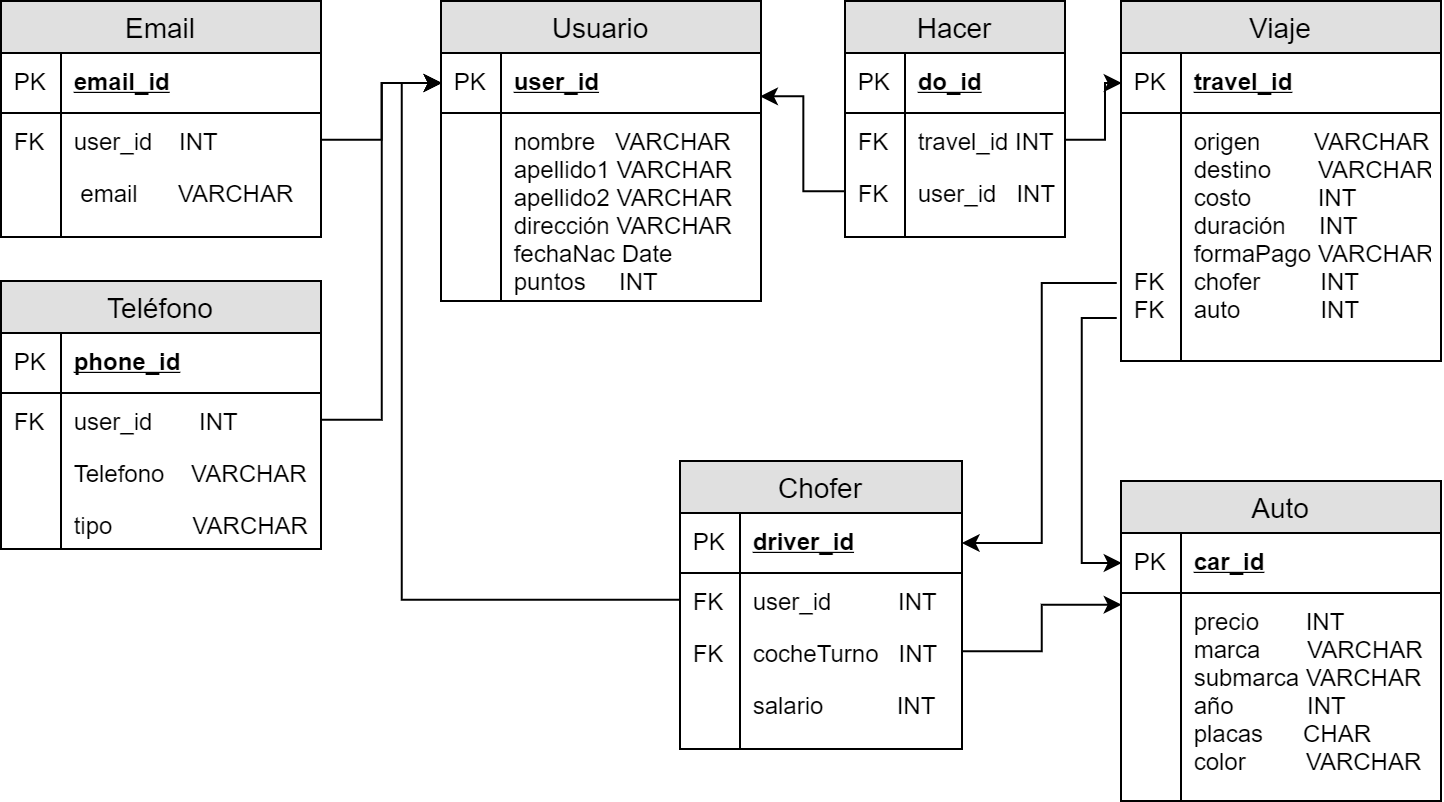
\includegraphics[scale=0.3]{1nf.png}
\caption{Diagrama relacional en 1NF}
\end{figure}
\textit{
Se crearon 2 nuevas tablas, email y phone, en la cual se guardarán los múltiples telefonos y correos de cada usuario, evitando así la redundacia de información de los Usuarios y cumpliendo así que todo campo no primario es dependiente funcionalmente de la llave primaria.}
\newpage
\section{Segunda Forma Normal}
Una relación está en 2FN si está en 1FN y si los atributos que no forman parte de ninguna clave dependen de forma completa de la clave principal. Es decir, que no existen dependencias parciales. Todos los atributos que no son clave principal deben depender únicamente de la clave principal.\par\null\par
Parafraseando un poco, significa que los atributos solo pueden depender de la llave primaria no de otro atributo, toda dependencia funcional, debe contener a la llave primaria del lado izquierdo.\par\null\par
Podría parecer que por ejemplo el costo, depende del origen, el destino y la duración, pero también depende de otros factores como la demanda, que no están en la tabla, entonces si es dependencia funcional solo de la llave primaria.\par\null\par
En las otras tablas no hay dependencias funcionales que no contengan a la llave primaria del lado izquierdo.\par\null\par
Donde no se cumple la regla es en la tabla \textbf{Auto}, ya que la marca depende funcionalmente de la submarca, por lo tanto debemos hacer otra tabla para esa dependencia funcional.
\begin{figure}[h!]
\centering
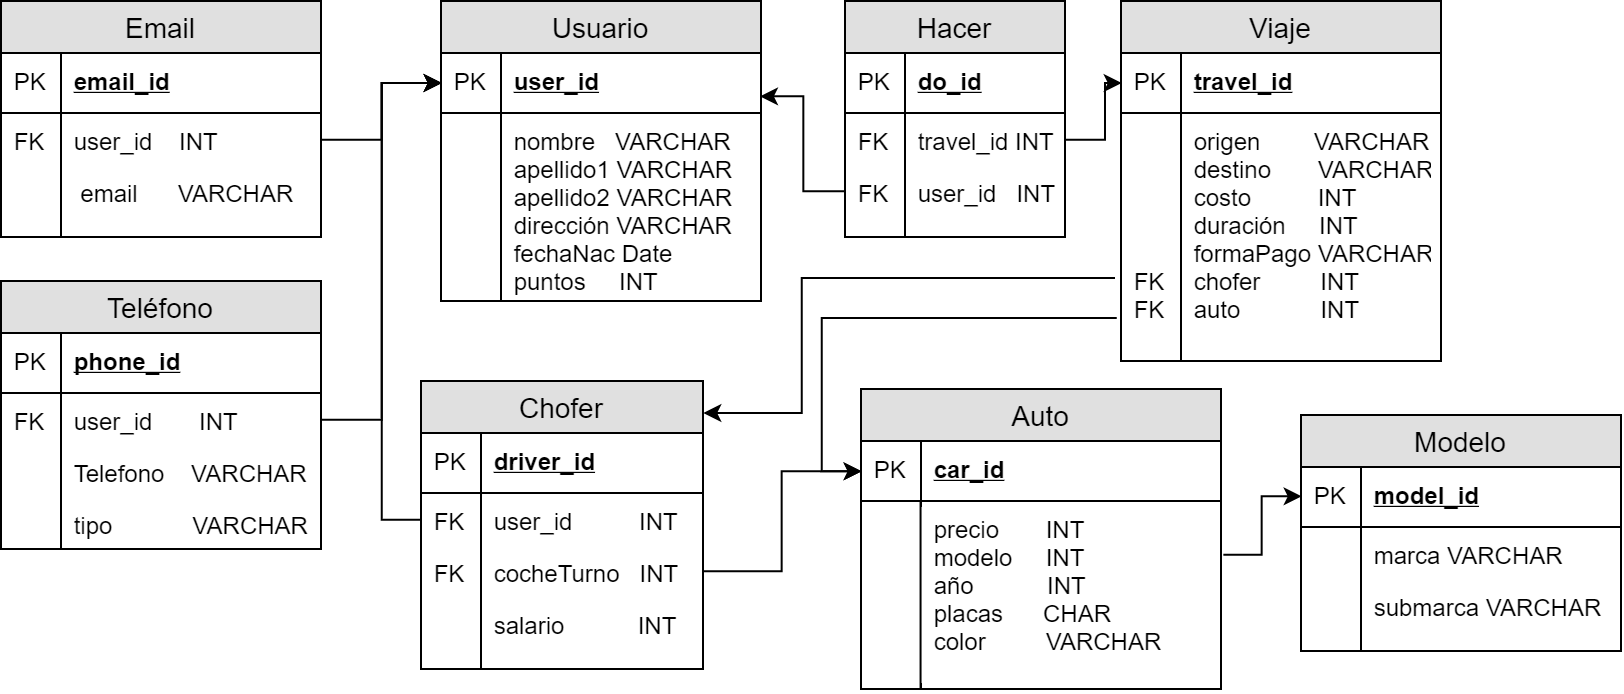
\includegraphics[scale=0.28]{2fn.png}
\caption{Diagrama relacional en 2NF}
\end{figure}
\newpage
\textit{Se agregó la tabla modelo, ya que la marca depende de la submarca, y esa dependencia funcional no tenía la llave primaria del lado izquierdo}
Por cuestión de practicidad se usá una llave primaria artificial, un entero autoincrementable, ya se explicó en el otro documento los argumentos, pero cuando se haga la traducción a SQL nos aseguraremos que la tupla (marca,submarca) sea no nula y única.


\section{Tercera Forma Normal}
“Una relación se encuentra en Tercera Forma Normal si, y solo si, se encuentra en 2FN y si los atributos no clave dependen de forma no transitiva de la clave primaria”
 \par\null\par
 La tabla ya cumplé la tercera forma normal, ya que no tiene dependencias transitivas, estas se quitaron en la anterior forma normal, por lo tanto podemos decir con seguridad que nuestro diagrama relacional \textbf{Está normalizada} 
 \begin{figure}[h!]
\centering
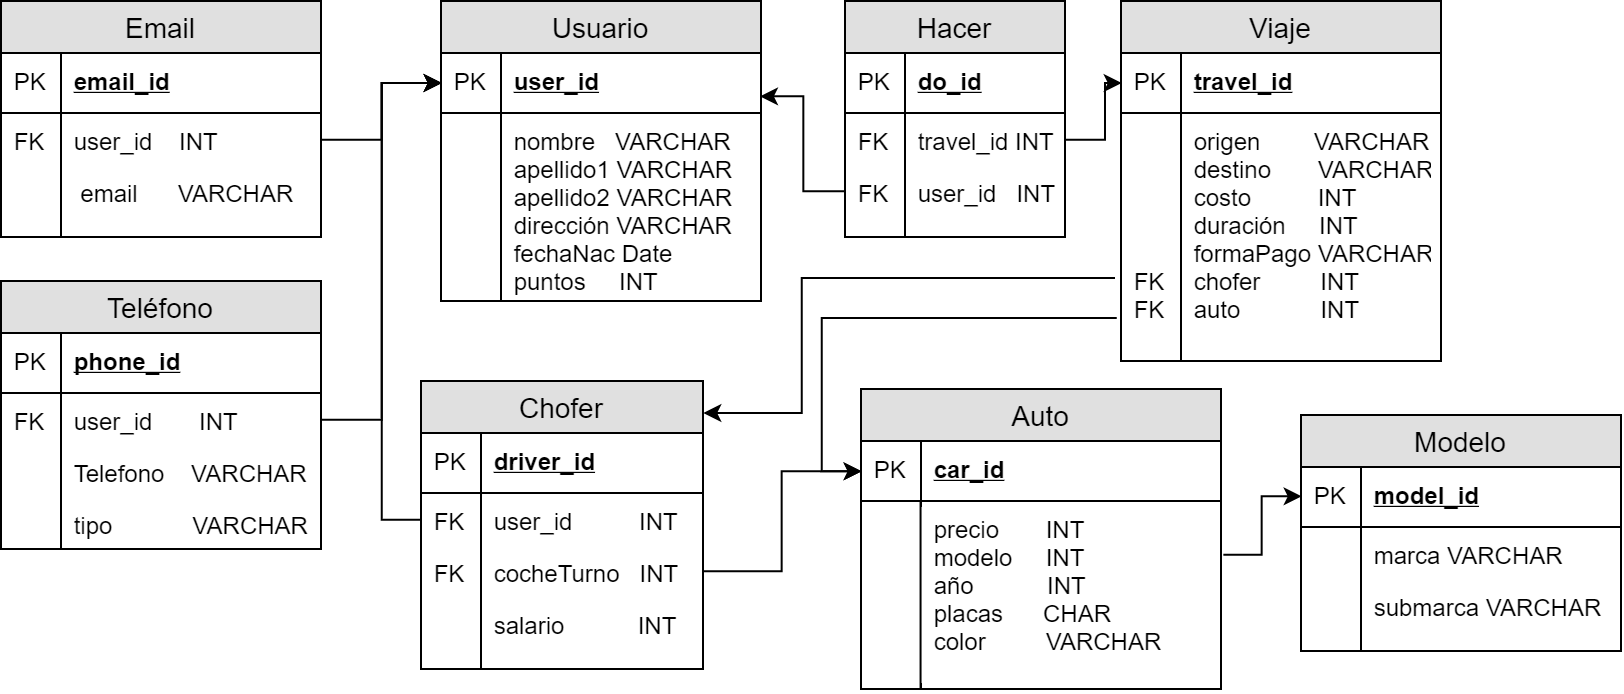
\includegraphics[scale=0.28]{2fn.png}
\caption{Diagrama relacional en 3FN}
\end{figure}
\end{document}
